% -----------------------------------------------
% Template for ICMC SMC 2014
% adapted and corrected from the template for SMC 2013,  which was adapted from that of  SMC 2012, which was adapted from that of SMC 2011
% -----------------------------------------------

\documentclass{article}
\usepackage{icmcsmc2014}
\usepackage{times}
\usepackage{ifpdf}
\usepackage[english]{babel}
\usepackage[utf8]{inputenc}
\usepackage{color}
\usepackage{amssymb}
\usepackage{amsmath}
%\usepackage{verbatim}
\usepackage{balance}
%\usepackage{cite}


\newenvironment{state}
{ \begin{list}
	{-}
	{	 \setlength{\leftmargin}{6mm}
	 	\setlength{\itemsep}{-3pt}}
}
{ \end{list} }

\definecolor{mygrey}		{gray}{0.98}
\newcommand{\defs}	[1]		{ 	\begin{center}\colorbox{mygrey}{
								\begin{minipage}[t]{0.99\columnwidth} 
								\ttfamily \small #1 
								\end{minipage}}\end{center}}

\newcommand{\verbcaption}[1]	{ \vspace{-5mm} \caption{#1}}

%%%%%%%%%%%%%%%%%%%%%%%% Some useful packages %%%%%%%%%%%%%%%%%%%%%%%%%%%%%%%
%%%%%%%%%%%%%%%%%%%%%%%% See related documentation %%%%%%%%%%%%%%%%%%%%%%%%%%
%\usepackage{amsmath} % popular packages from Am. Math. Soc. Please use the 
%\usepackage{amssymb} % related math environments (split, subequation, cases,
%\usepackage{amsfonts}% multline, etc.)
%\usepackage{bm}      % Bold Math package, defines the command \bf{}
%\usepackage{paralist}% extended list environments
%%subfig.sty is the modern replacement for subfigure.sty. However, subfig.sty 
%%requires and automatically loads caption.sty which overrides class handling 
%%of captions. To prevent this problem, preload caption.sty with caption=false 
%\usepackage[caption=false]{caption}
%\usepackage[font=footnotesize]{subfig}


%user defined variables
\def\papertitle{Representation of Musical Computer Processes}
\def\firstauthor{D. Fober}
\def\secondauthor{Y. Orlarey}
\def\thirdauthor{S. Letz}
\def\allauthors{Dominique Fober, Yann Orlarey, Stéphane Letz}

% adds the automatic
% Saves a lot of ouptut space in PDF... after conversion with the distiller
% Delete if you cannot get PS fonts working on your system.

% pdf-tex settings: detect automatically if run by latex or pdflatex
\newif\ifpdf
\ifx\pdfoutput\relax
\else
   \ifcase\pdfoutput
      \pdffalse
   \else
      \pdftrue
\fi

\ifpdf % compiling with pdflatex
  \usepackage[pdftex,
    pdftitle={\papertitle},
    pdfauthor={\firstauthor, \secondauthor, \thirdauthor},
    bookmarksnumbered, % use section numbers with bookmarks
    pdfstartview=XYZ % start with zoom=100% instead of full screen; 
                     % especially useful if working with a big screen :-)
   ]{hyperref}
  %\pdfcompresslevel=9

  \usepackage[pdftex]{graphicx}
  % declare the path(s) where your graphic files are and their extensions so 
  %you won't have to specify these with every instance of \includegraphics
  \graphicspath{{./figures/}}
  \DeclareGraphicsExtensions{.pdf,.jpeg,.png}

  \usepackage[figure,table]{hypcap}

\else % compiling with latex
  \usepackage[dvips,
    bookmarksnumbered, % use section numbers with bookmarks
    pdfstartview=XYZ % start with zoom=100% instead of full screen
  ]{hyperref}  % hyperrefs are active in the pdf file after conversion

  \usepackage[dvips]{epsfig,graphicx}
  % declare the path(s) where your graphic files are and their extensions so 
  %you won't have to specify these with every instance of \includegraphics
  \graphicspath{{./figures/}}
  \DeclareGraphicsExtensions{.eps}

  \usepackage[figure,table]{hypcap}
\fi

%setup the hyperref package - make the links black without a surrounding frame
\hypersetup{
    colorlinks,%
    citecolor=black,%
    filecolor=black,%
    linkcolor=black,%
    urlcolor=black
}


% Title.
% ------
\title{\papertitle}

% Authors
% Please note that submissions are NOT anonymous, therefore 
% authors' names have to be VISIBLE in your manuscript. 
%
% Single address
% To use with only one author or several with the same address
% ---------------
\oneauthor
   {\allauthors} {GRAME \\ Centre national de création musicale \\ Lyon, France \\ %
     {\tt \href{mailto:fober@grame.fr}{fober@grame.fr} \href{mailto:orlarey@grame.fr}{orlarey@grame.fr} \href{mailto:letz@grame.fr}{letz@grame.fr}}}

%Two addresses
%--------------
% \twoauthors
%   {\firstauthor} {Affiliation1 \\ %
%     {\tt \href{mailto:author1@smcnetwork.org}{author1@smcnetwork.org}}}
%   {\secondauthor} {Affiliation2 \\ %
%     {\tt \href{mailto:author2@smcnetwork.org}{author2@smcnetwork.org}}}

% Three addresses
% --------------
% \threeauthors
%   {\firstauthor} {GRAME, Lyon, France \\ %
%     {\tt \href{mailto:fober@grame.fr}{fober@grame.fr}}}
%   {\secondauthor} {Affiliation2 \\ %
%     {\tt \href{mailto:author2@smcnetwork.org}{author2@smcnetwork.org}}}
%   {\thirdauthor} { Affiliation3 \\ %
%     {\tt \href{mailto:author3@smcnetwork.org}{author3@smcnetwork.org}}}


% ***************************************** the document starts here ***************
\begin{document}
%
\capstartfalse
\maketitle
\capstarttrue
%
\begin{abstract}
The paper presents a study about the representation of musical computer processes within a music score. The idea is to provide performers with information that could be useful especially in the context of interactive music. The paper starts with a characterization of a musical computer process in order to define the \emph{values} to be represented. Next it proposes an approach to time representation suitable to asynchronous processes representation.
\end{abstract}
%

%----------------------------------------------------------------
\section{Introduction}\label{sec:intro}
%----------------------------------------------------------------
Throughout the last decades, the development of electronic and digital technologies, including sound production, gesture captation, has led to a musical revolution and to the emergence of new genres firmly established in the culture and musical imagination.
From these evolutions, new needs have emerged, notably in terms of music notation and representation \cite{freeman11}. Raised by artistic forms like \emph{interactive music} or \emph{live coding}, questions related to dynamic notation or musical process representation are taking a significant importance. With interactive music, the cohabitation between static scores and interaction processes is to be organized. With live coding, the border between programmation and score tends to be blurry \cite{magnuss11}.
Today, the object of the musical notation needs to be redefined to take account of the new dimensions of the current artistic practices.

This paper addresses the dynamic representation of processes and their states in the single graphical space of the musical score. 

The musical context gives a specific dimension to the problematic of a process representation, because we are interrested in its current state, but also in a set of time ordered states, including possible future states. Usability constraints require these state to be readable in real-time, i.e. in the time of the score performance, and to be a guide for the interaction choices of the performer.

The objective of the study is to integrate the representation of processes to INScore \cite{Fober:12a,Fober:13b}, an environment for the design of augmented interactive music score. 

We will first present existing approaches in the domain of process representation, with a viewpoint centered on musical applications. We will next define the elements to characterize an interaction process. We will finally propose a model of process representation, not in the graphic space - that remains the score domain and the composer responsibility - but in terms of communication between the tools involved in a piece realization.

%----------------------------------------------------------------
\section{Existing approaches}
%----------------------------------------------------------------
Generally provided with operating systems, there are tools to visualize the system state in terms of resources usage: CPU, memory, network bandwith, etc. (figure \ref{fig:sys}). 
In the musical domain, tools for music computation are proposing similar representations: the system state may include both the application resources usage and the system parameters, generaly reflecting audio processes.

\begin{figure}[h]
\begin{center}
	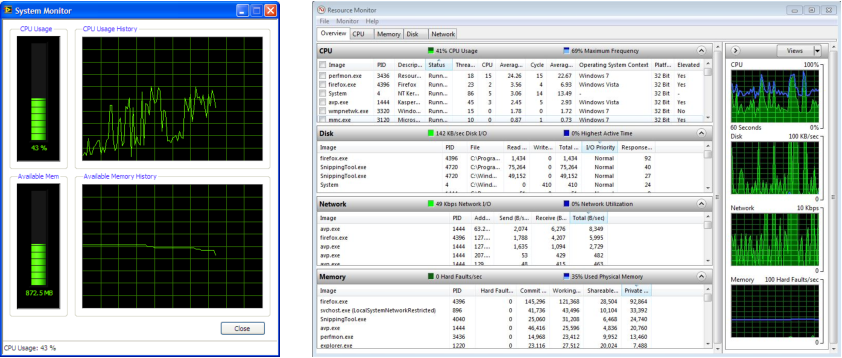
\includegraphics[width=0.9\columnwidth]{imgs/system}
\caption{Visualization of the system state under Windows}
\label{fig:sys}
\end{center}
\end{figure}

In the musical domain, PureData \cite{Puckette96puredata} and Max/MSP \cite{puckette91} are among the applications frequently used for interactive music design. PureData provides rough tools to represent the system state (figure \ref{fig:maxpd}b). Max/MSP includes an audio resources monitor (figure \ref{fig:maxpd}a) that gives also the value of the audio setup, like sampling rate, I/O vector size, etc.

\begin{figure}[h]
\begin{center}
	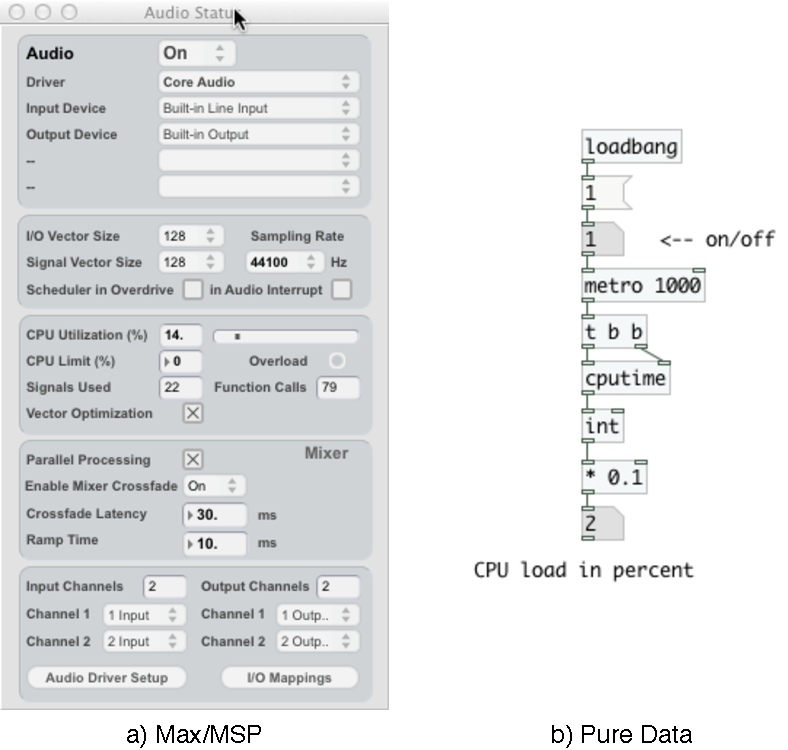
\includegraphics[width=0.75\columnwidth]{imgs/max-pd}
\caption{Visualization of the system state with Max/MSP and Pure Data}
\label{fig:maxpd}
\end{center}
\end{figure}

In the context of interactive music, the current position in the score is part of the system state but the notion of score is missing win tools like Max/MSP or PureData. Extensions like Bach \cite{agostini12b} or MAXScore \cite{didko08} allow to introduce the music notation in Max/MSP, but without taking account of the musical processes representation.

With environments like Open Music \cite{Assayag:1999:CCI:1116106.1116119} or i-score \cite{AllombertDA08}, a process is viewed as an \emph{opaque} box. Its temporal dimension is taken into account and a cursor locates its current time position, but without more information about the process activity.

That's in the domain of live coding and interactive systems that the approaches look the more advanced. 
Thor Magnusson is developping a thought and tools that tend to narrow programming and music score \cite{magnusson:07,magnuss11}.
Ge Wang proposes also an approach based on code \cite{Wang04on-the-flyprogramming:} as factor of instrumental expression for the \emph{live coding}, with the programming language Chuck \cite{Wang03chuck:a}. This idea is notably implemented in the audio programming environment  \emph{The Audicle} \cite{Wang04theaudicle} where different visualizations of the code and of the system activity are proposed in an original and extensible approach(figure \ref{fig:audicle}).

\begin{figure}[h]
\begin{center}
	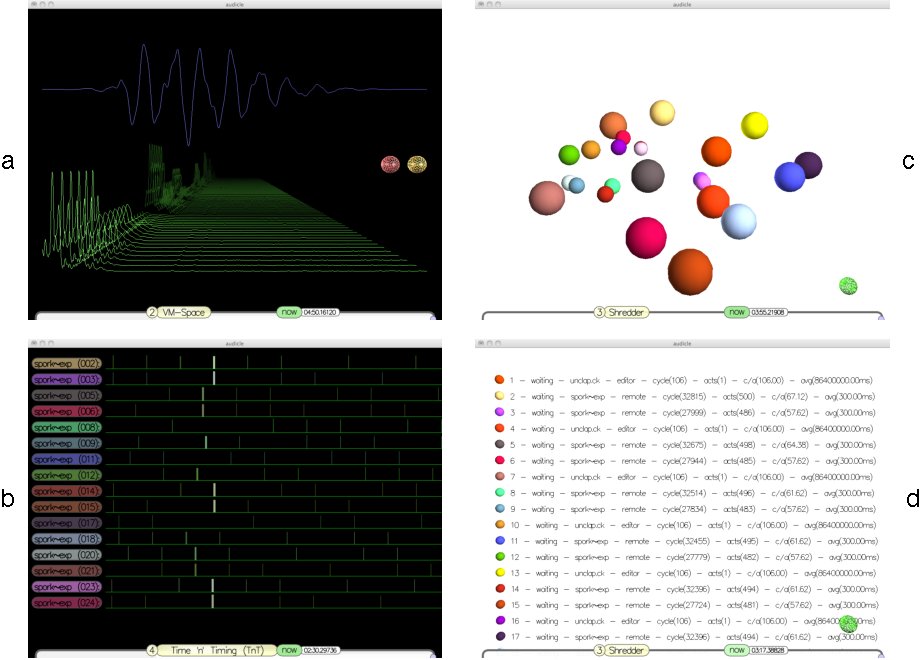
\includegraphics[width=0.9\columnwidth]{imgs/audicle}
\caption{Visualization of the system state in the Audicle : 
a) waveform and spectrum, b) temporal information per thread, 
c) threads activity in a graphic form, d) in a detailled textual form.}
\label{fig:audicle}
\end{center}
\end{figure}

Another approach of the visualization is centered on the listener, aiming at improving the perception using graphical information in a live coding context \cite{McLean:2010:VLC:2227180.2227185} or to make the mechanism of electronic instruments perceptible \cite{berthaut13} (figure \ref{fig:rouages}).

\begin{figure}[h]
\begin{center}
	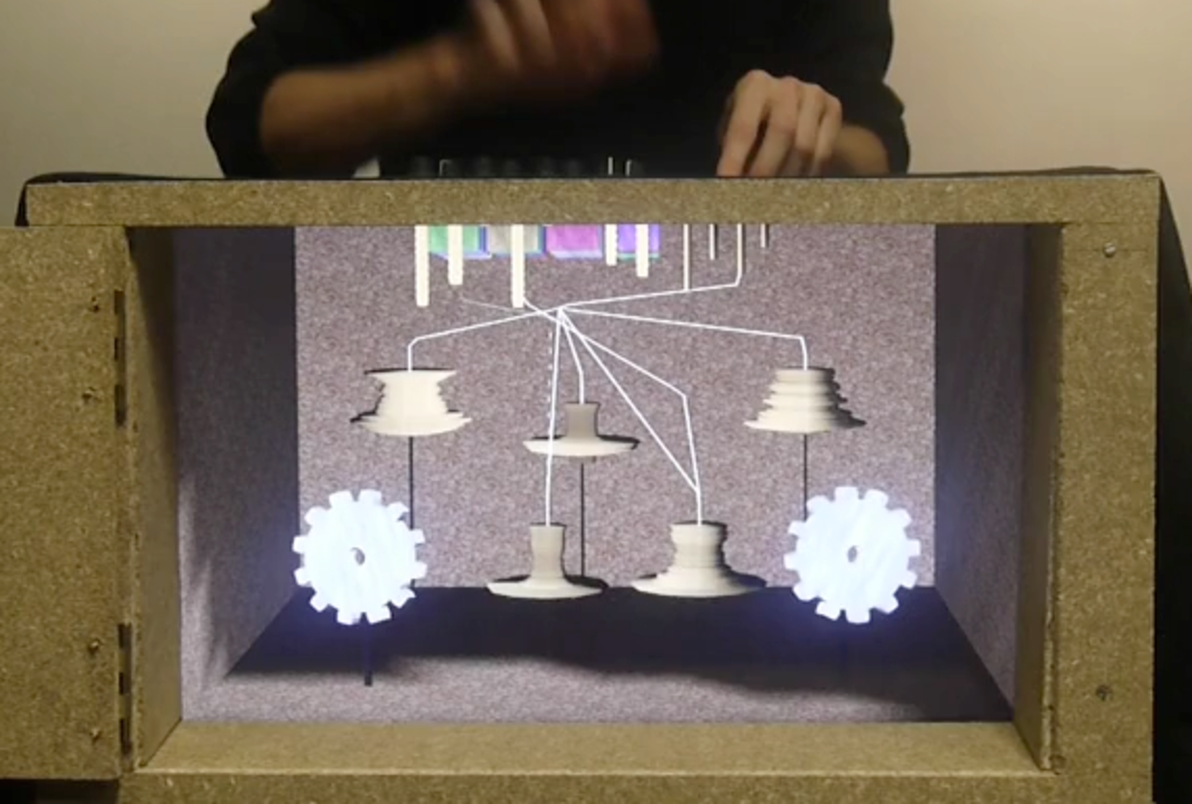
\includegraphics[width=0.8\columnwidth]{imgs/rouages}
\caption{Visualization electronic instruments mechanism.}
\label{fig:rouages}
\end{center}
\end{figure}

The main limitation of all these approaches is to be partial and centered on the applications that propose them. In addition, there is no emergent general model and the interoperability between the tools is not taken into account.


%----------------------------------------------------------------
\section{Characterization of a musical computer process}
%----------------------------------------------------------------
We will consider music computer processes as resulting from the music composition and thus, as being part of the music score. From this viewpoint, a process takes place in time: it can be passed, present or future. We will talk of \emph{active} process for a process that is present, and of \emph{inactive} process for a past or future process.

The temporal status will determine different ways to characterize a process: the properties of a process will be different whether active or inactive. Similarly, properties of a past process will differ from those of a future process, which date and duration may be undefined, relative to an external event.

The characterization of a musical computer process we will be based on three types of information, classified according to their change rate:
\begin{itemize}%\itemsep2pt
\item a static state: represent the information that doesn't change (e.g. the parent process) or that may change at a low rate (e.g. the sampling freq.)
\item a dynamic state: represents the information that changes over time and depend on the process execution (e.g. the CPU usage)
\item a temporal state: the process start date and its end date or duration. These properties may be undefined in an interactive context.
\end{itemize}


\subsection{Static state}
%------------------------------------------------------------
A process static state is made of the set of information that are invariant or that change at a low rate. This state is completely defined for an active process. It reflects the last active state for a passed process. For a future process, it may indicate the first state to activate when it is known in advance.

For a generic process, the state may include:
\begin{state}
\item its parent process
\item its status (active | inactive)
\item its computation mode (vectorization, parallélization,...)
\item ...
\end{state}

For an audio process, the state may include:
\begin{state}
\item the I/O buffers size
\item the sampling rate
\item the I/O devices
\item the driver
\item ...
\end{state}

For any process, the state may include the value of the control parameters. For example: delay and feedback values of an echo.

The set of static properties is process dependant.


\subsection{Dynamic state}
%------------------------------------------------------------
The dynamic state of a process is closely linked to its activity and characterizes an active process.

For a generic process, the state may include:
\begin{state}
\item the CPU usage
\item the threads count
\item the memory usage
\item ...
\end{state}

The result of a process computation may also reflect its state, e.g. the values of a process that computes a signal.

The dynamic state may include indications on the current computation, e.g. an index of confidence for a process that is doing pitch recognition or that is doing score following.

The set of dynamic properties is process dependant.


\subsection{Temporal state}
%------------------------------------------------------------

In a musical context and especially for interactive music \cite{Rowe:1992:IMS:530519}, the temporal state of process (i.e. its start date, its end date or its duration) may be partially or totally undefined. 

In case of an active process, the start date is known but its end may depend on another process and/or an external event. For a future process, both the start and end dates may be undefined.

In addition, the way to represent dates and durations may lead to undefined results, e.g. when expressed in a time relative to a tempo that is undefined.

In a musical context, this temporal information is critical for the performance of a piece and thus, require to be represented whatever its status.

The temporal properties are common to all the processes.


%----------------------------------------------------------------
\section{Representing the state of a musical computer process}
%----------------------------------------------------------------
We propose a format to represent the state of a musical process, suitable to inter-applications collaboration, allowing to dissociate a process involved in a piece computation and its graphic representation, that could be viewed as part of the music score.

We define the state of a process as a set of values that characterise this process at a given time.
We'll talk of \emph{property} to refer to one of these values. To represent a process state, this process should be able to describe its properties set.


\subsection{Definition of a property}
%------------------------------------------------------------
A process property is the association of an identifier and a value that may change over time. The value may be a number or a vector of values: e.g. a space position is defined by 3 values.

The value of a property may be bounded by an interval. Finally, the frequency of a property variation may also be defined.

The type of the values is in:
\begin{state}
\item \textbf{int} : for an integer number 
\item \textbf{float} : for a floating point number
\item \textbf{bool} : for a boolean 
\item \textbf{probability} : the value is a probability. By convention, it will be expressed by floating point numbers in the interval [0, 1]. 
\end{state}
Values of a \textbf{vector} type are defined by a list of types.

\begin{figure}[h]
{\small 
\begin{verbatim}
 property : ident type [ range freq ]
 ident    : string
          | url
 freq     : integer
 type     : 'int'
          | 'float'
          | 'bool'
          | 'probability'
          | ( vector )
 vector 	 : type
          | vector type
 range    : value value
 value    : int
          | float
          | bool
          | ( vlist )
 vlist    : value
          | vlist value
\end{verbatim}
}
\verbcaption{A property definition}
\label{fig:caract}
\end{figure}

By convention, the frequency defines the rate of a value variation: it indicates a number of changes by second. The value $0$ denotes constant values. When the variation rate is unknown, the frequency should be omitted.


\subsection{Declaration of a properties set}
%------------------------------------------------------------
A process state is defined by a list of properties (figure \ref{fig:state}). In order to represent this state, a process must be able to communicate a description of its state.

\begin{figure}[h]
{\small 
\begin{verbatim}
 process-state : states
 states        : property
               | states property
\end{verbatim}
}
\verbcaption{Description of a process state}
\label{fig:state}
\end{figure}

JSON \cite{json} could be used to declare the properties of a process. The figure \ref{fig:karplus} gives the example of a FAUST  \cite{orlarey:09c} process which state include the value of the control parameters as well as the computed signal.

%\vspace{-15mm}
\begin{figure}[h]
{\small
\begin{verbatim}
{
  "process": "karplus",
  "states": [
   {
     "ident": "excitation",
     "type" : "float",
     "range": [{"min": 2},{"max": 512}]
   },
   {
     "ident": "play",
     "type" : "bool"
   },
   {
     "ident": "level",
     "type" : "float",
     "range": [{"min": 0},{"max": 1}]
   },
   {
     "ident": "attenuation",
     "type" : "float",
     "range": [{"min": 0},{"max": 1}]
   },
   {
     "ident": "duration",
     "type" : "float",
     "range": [{"min": 2},{"max": 512}]
   },
   {
     "ident": "signal",
     "type" : "float",
     "range": [{"min": -1},{"max": 1}],
     "freq" : 44100
   }
  ]
}
\end{verbatim}
}
\verbcaption{A FAUST process described using JSON}
\label{fig:karplus}
\end{figure}

%\vspace{-20mm}

\subsection{A property state}
%------------------------------------------------------------
The state of a property will be send as a pair associating an identifier and its value.

\begin{figure}[h]
\defs{
\{ "excitation" : 124 \}
}
\verbcaption{Value of the \texttt{excitation} of the process \texttt{karplus} using the JSON format}
\label{fig:excit}
\end{figure}

When a list of values is associated to an identifier (figure \ref{fig:sign}), they could be interpreted in the context of the property frequency: when a frequency is defined, the set of values takes the corresponding duration.
\begin{figure}[h]
\defs{
 \{ "signal" : [ -0.2, 0.1, 0.23, -0.05, -0.01, 0.8, 0.8, 0.02, -0.5 ]  \}
}
\verbcaption{Values of the \texttt{signal} computed by the process \texttt{karplus}}
\label{fig:sign}
\end{figure}

OSC \cite{OSC} may be used to transmit a state. In this case, the OSC address could be used as identifier (figure \ref{fig:osc})
\begin{figure}[h]
\defs{
 /karplus/signal -0.2  0.1  0.23  -0.05  -0.01  0.8  0.8  0.02  -0.5
}
\verbcaption{Values of the \texttt{signal} transmitted via OSC}
\label{fig:osc}
\end{figure}


\subsection{Temporal state representation}
%------------------------------------------------------------
All the processes have two common properties: a start date and a duration (or end date). These properties may be undefined (e.g. for a future process), or partially defined (e.g. for an active process which end date is undefined).

In the context of interactive music, an undefined date corresponds to an external event. For example,
\begin{state}
\item a process start or end may correspond to the start or end of an improvisation sequence,
\item a process mey be conditionally triggered, e.g. when a specific note sequence is played or in case of silence.
\end{state}
More generally, the scheduling of such processes may be described in terms of Allen relations \cite{Allen:1983:MKT:182.358434}, relatively to the events which they depend on. We will talk of \emph{event based date or duration} to refer to these undefined dates or durations.

The properties of a process temporal state are described by a start and an end or duration (figure \ref{fig:time}). The values can be expressed as time or under event form. 
\begin{figure}[h]
\defs{
process-temporal-state 

\ \ \ \ \ \ : begin  [ end | dur ] \\
begin : time | event \\
end \ \ : time | event \\
dur \ \ : time | event 
}
\verbcaption{Properties of a process temporal state}
\label{fig:time}
\end{figure}



%----------------------------------------------------------------
\subsubsection{Events representation}

Even when a process has an event based date, we would like to represent it, at least in an approximative manner. In order to provide support for such representation, an event based date is defined as a triplet $\mathcal{T} = ( t_{left},\ t,\ t_{right} )$, associated to a confidence level  $\mathcal{P}$  and followed by an optionnal label  (figure \ref{fig:evtime}). 

$\mathcal{T}$ is such that $t_{left} \leqslant t \leqslant t_{right}$. $\mathcal{T}$ defines a realisation interval $[t_{left},\ t_{right}]$ and a possible realisation date $t$. The confidence level  $[t_{left},\ t_{right}]$ represents the realisation likelihood of the event at the date $t$. It is expressed as a floating point value in the interval 0, 1.

\begin{figure}[h]
\defs{
event \ \ \ \ \ :  timeset confidence [ label ] \\
timeset \ \ \ :  ( leftbound, expected, rightbound ) \\
leftbound \ : time \\
expected \ \ : time \\
rightbound : time 
}
\verbcaption{Approximation of event based time.}
\label{fig:evtime}
\end{figure}

This kind of representation is intermediate between the description of Allen relations and classical dating. As an example, the following relation {\small \texttt{A m (B si (C fi D))}} expressed in terms of Allen relations (figure \ref{fig:arel}) could be expressed in a \emph{semi-instanciated} way as follows:
{\small \begin{verbatim}
 {   "process": "A",
     "start": "0/1",
     "dur": [ "1/4", "1/2", "1/1", 0.7 ]
 }
 {   "process": "B",
     "start": [ "1/4", "1/2", "1/1", 0.7 ],
     "dur": "1/4"
 }
 {   "process": "C",
     "start": [ "1/4", "1/2", "1/1", 0.7 ],
     "dur":   [ "1/2", "3/4", "1/1", 0.7 ]
 }
 {   "process": "D",
     "start": [ "0/1", "1/2", "1/2", 0.8 ],
     "end":   [ "3/4", "5/4", "3/2", 0.5 ]
 }
\end{verbatim}
}

\begin{figure}[h]
\begin{center}
	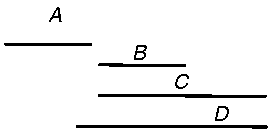
\includegraphics[width=0.5\columnwidth]{imgs/relation}
\caption{Relations between 4 processes: B and C start with the end of A, D ends with C.}
\label{fig:arel}
\end{center}
\end{figure}

Note that the start date of the process $D$ expresses a constraint on the duration, that should be greater or equal to a whole note.

One of the possibilities for the representation may consist to use a color gradient to account for uncertainties, as illustrated in figure \ref{fig:exvue}, that is based on the example above.

\begin{figure}[h]
\begin{center}
	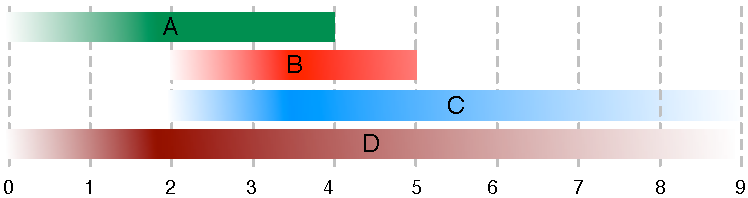
\includegraphics[width=0.8\columnwidth]{imgs/exemplevue}
\caption{Representation of the processes A, B, C, D, using color gradients to account for uncertainties.}
\label{fig:exvue}
\end{center}
\end{figure}

%----------------------------------------------------------------
\section{Conclusion}
%----------------------------------------------------------------
We propose a simple description of a musical process state. This description is disconnected from any representation format or communication protocol. However, examples using JSON or OSC are given because their simplicity of implementation was consistent with the proposed description of musical processes.

The critical problem of the representation of event based time is treated using a \emph{probabilistic semi-instantiated} approach. This solution is less general than a description in terms or Allen relations, but it avoids solving the corresponding constraints to visualization applications, while realization systems have already to do it.

\begin{acknowledgments}
This research has been conducted in the framework of the INEDIT project that is funded by the French National Research Agency [ANR-12-CORD-009].
\end{acknowledgments} 

\balance
\bibliography{../interlude}

\end{document}
